\chapter{Содержание работы}
\textit{Цель работы}:  построение доверительных интервалов для математического ожидания и дисперсии нормальной случайной величины
\begin{enumerate}[wide=0pt]
	\item Для выборки объема n из генеральной совокупности X реализовать в виде программы на ЭВМ:
	\begin{enumerate}
		\item вычисление точечных оценок $\hat\mu(\vec X_n)$ и $S^2(\vec X_n)$ математического ожидания $MX$ и дисперсии $DX$ соответственно;
		\item вычисление нижней и верхней границ $\underline\mu(\vec X_n)$, $\overline\mu(\vec X_n)$ для $\gamma$-доверительного интервала для математического ожидания $MX$;
		\item вычисление оценок $\hat{\mu}$ и $S^2$ математического ожидания MX и дисперсии DX;
		\item вычисление нижней и верхней границ $\underline\sigma^2(\vec X_n)$, $\overline\sigma^2(\vec X_n)$ для $\gamma$-доверительного интервала для дисперсии $DX$;
	\end{enumerate}
	\item вычислить $\hat\mu$ и $S^2$ для выборки из индивидуального варианта;
	\item для заданного пользователем уровня доверия $\gamma$ и $N$ – объёма выборки из индивидуального варианта:
	\begin{enumerate}
		\item на координатной плоскости $Oyn$ построить прямую $y = \hat\mu(\vec{x_N})$, также графики функций $y = \hat\mu(\vec x_n)$, $y = \underline\mu(\vec x_n)$ и $y = \overline\mu(\vec x_n)$ как функций объема $n$ выборки, где $n$ изменяется от 1 до $N$;
		\item на другой координатной плоскости $Ozn$ построить прямую $z = S^2(\vec{x_N})$, также графики функций $z = S^2(\vec x_n)$, $z = \underline\sigma^2(\vec x_n)$ и $z = \overline\sigma^2(\vec x_n)$ как функций объема $n$ выборки, где $n$ изменяется от 1 до $N$.
	\end{enumerate}
\end{enumerate}

\chapter{Теоретические сведения}
Интервальная оценка позволяет получить вероятностную характеристику точности оценивания неизвестного параметра.
Пусть $\vec X_n$ -- случайная выборка объёма $n$ из генеральной совокупности $\vec{X}$ с функцией распределения $F(x; \theta)$, зависящей от параметра $\theta$, значение которого неизвестно. Предположим, для параметра  $\theta$ был построен интервал $(\underline{\theta}(\vec{X}), \overline{\theta}(\vec{X}))$, где $\underline{\theta}(\vec{X})$ и $\overline{\theta}(\vec{X})$ являются функциями случайной выборки $\vec{X_n}$, таким чтобы выполнялось равенство: 

\begin{equation}
P\{\underline{\theta}(\vec X)< \theta< \overline{\theta}(\vec X)\}=\gamma
\end{equation} 

Интервал $\theta(\vec X_n), \theta(\vec -X_n)$ называют доверительным интервалом для параметра $\theta$ с коэффициентом доверия $\gamma$ или $\theta$-доверительным интервалом.

Пусть известно, что у случайной величины нормальное распределение. 
Тогда в зависимости от известных параметров случайной величины можно построить доверительную оценку для неизвестных параметров системы.

\section*{Доверительная оценка для математического ожидания при известной дисперсии}
Пусть $\vec{X_n} = (X_1, ..., X_n)$ -- случайная выборка объёма n из генеральной совокупности X, распределенной по нормальному закону с параметрами $\mu и \sigma^2$, $\sigma^2$ известна.  

В этом случае статистика $\frac{\overline{X} - \mu}{\sigma}*\sqrt{n}$ имеет стандартное нормальное распределение.
Поэтому:
\begin{equation}
P\{-u_{1 - \alpha} < \frac{\overline{X} - \mu}{\sigma}*\sqrt{n} <  u_{1 - \alpha}\} = 1 - 2\alpha
\end{equation}

\section*{Доверительная оценка для математического ожидания при неизвестной дисперсии}
При неизвестной дисперсии $\sigma^2$ статистика
\begin{equation}
\frac{\overline{X} - \mu}{S{\vec{X_n}}}*\sqrt{n}
\end{equation}
имеет распределение Стьюдента с n - 1 степенью свободы.

Поэтому нижнюю границу можно определить так:
\begin{equation}
\underline{\mu} = \overline{X} - \frac{S(\vec{X_n})}{\sqrt{n}}t_{1 - \alpha}(n - 1)
\end{equation}

А верхнюю границу можно определить так:
\begin{equation}
\overline{\mu} = \overline{X} + \frac{S(\vec{X_n})}{\sqrt{n}}t_{1 - \alpha}(n - 1)
\end{equation}

В случае лабораторной работы используется именно этот вариант построения доверительного интервала.

\section*{Доверительная оценка для дисперсии при неизвестном математическом ожидании}
В этом случае статистика
\begin{equation}
\frac{(n - 1)S^2(\vec{X_n})}{\sigma^2}
\end{equation}

имеет $\chi^2$-распределение с $n - 1$ степенью свободы.

Поэтому доверительный интервал можно представить как:
\begin{equation}
P\{\frac{(n- 1)S^2(\vec{X_n})}{\chi^2_{1 - \alpha} * (n - 1)} < \sigma^2 < \frac{(n- 1)S^2(\vec{X_n})}{\chi^2_{\alpha} * (n - 1)} \}
\end{equation}
 
\chapter*{Код программы}
На листинге 1 представлен код программы:
\FloatBarrier
\begin{lstinputlisting}{src/main.m}
\end{lstinputlisting}
\FloatBarrier

\chapter*{Результаты работы программы}
На рисунке 1 представлен график функции точечных и интервальных оценок для математического ожидания:
\FloatBarrier
\begin{figure}[h]
	\begin{center}
		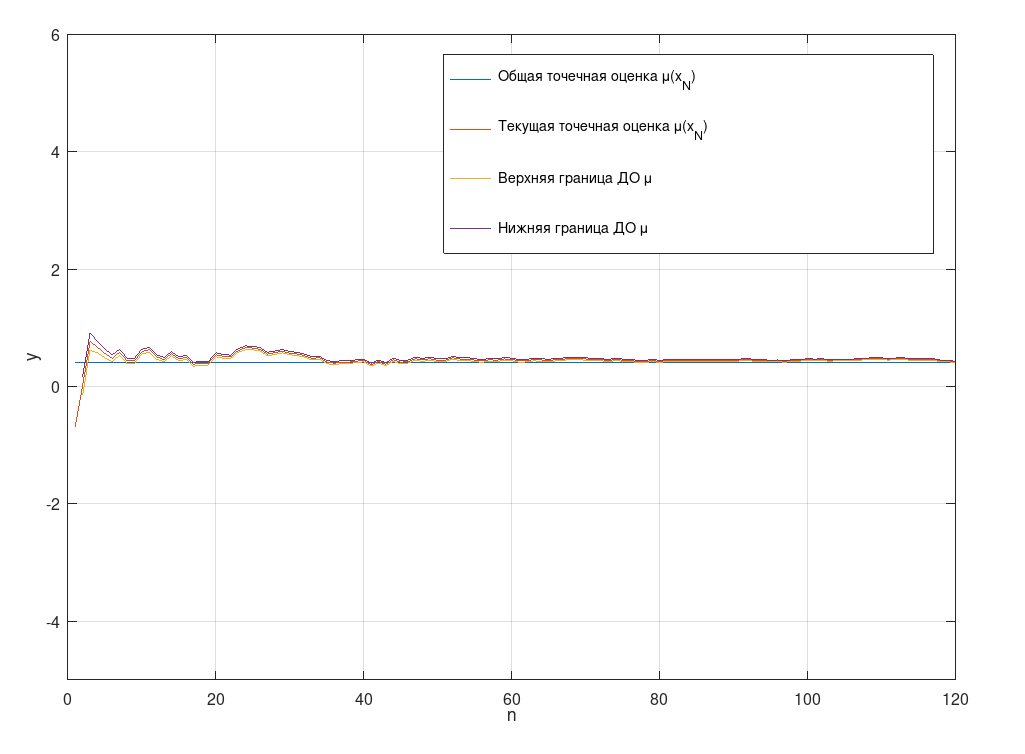
\includegraphics[width=\linewidth, height=12cm]{inc/mu.png}
	\end{center}
\end{figure}
\FloatBarrier

\newpage

На рисунке 2 представлен график функции точечных и интервальных оценок для дисперсии:
\FloatBarrier
\begin{figure}[h]
	\begin{center}
		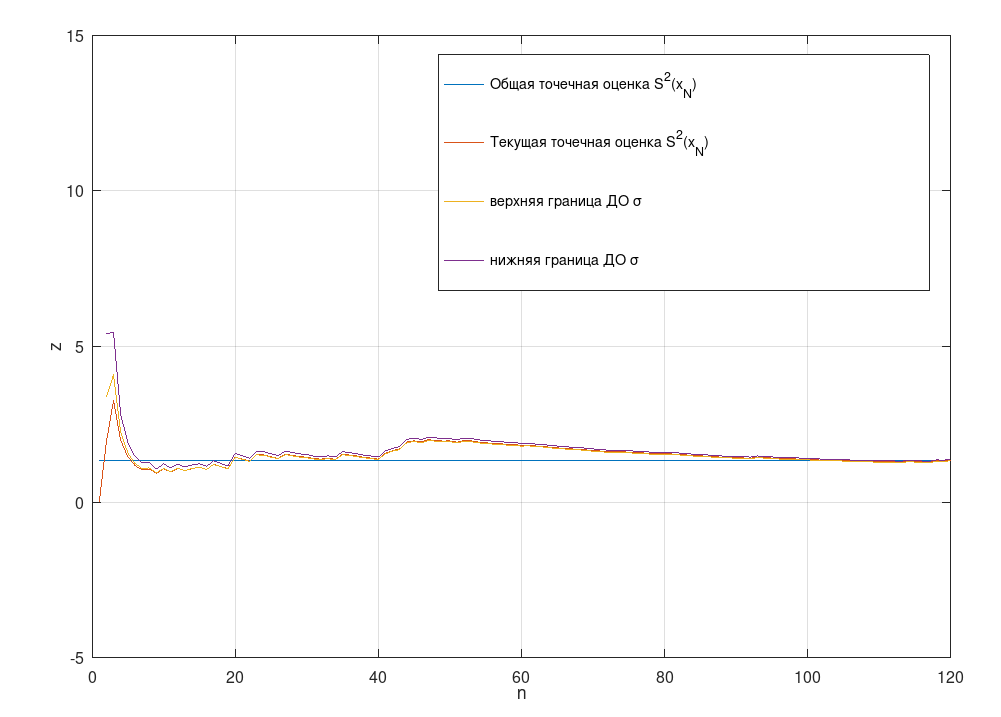
\includegraphics[width=\linewidth, height=12cm]{inc/s2.png}
	\end{center}
\end{figure}
\FloatBarrier

Результат работы программы представлен на рисунке 3:
\FloatBarrier
\begin{figure}[h]
	\begin{center}
		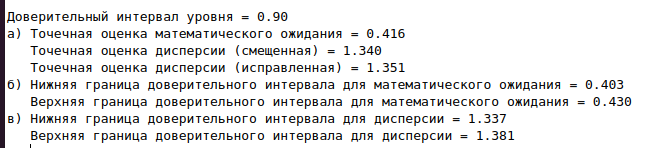
\includegraphics[width=\linewidth]{inc/result.png}
	\end{center}
\end{figure}
\FloatBarrier
